\chapter{Estimating DSGE models - advanced topics} \label{ch:estadv}

This chapter focusses on advanced topics and features of Dynare in the area of model estimation. The chapter begins by presenting a more complex example than the one used for illustration purposes in chapter \ref{ch:estbase}. The goal is to show how Dynare would be used in the more ``realistic'' setting of reproducing a recent academic paper. The chapter then follows with sections on comparing models to one another, and then to BVARs, and ends with a table summarizing where output series are stored and how these can be retrieved. \\


\section{Alternative and non-stationary example}
The example provided in chapter \ref{ch:estbase} is really only useful for illustration purposes. So we thought you would enjoy (and continue learning from!) a more realistic example which reproduces the work in a recent - and highly regarded - academic paper. The example shows how to use Dynare in a more realistic setting, while emphasizing techniques to deal with non-stationary observations and stochastic trends in dynamics. \\

\subsection{Introducing the example}
The example is drawn from \citet{Schorfheide2000}. This first section introduces the model, its basic intuitions and equations. We will then see in subsequent sections how to estimate it using Dynare. Note that the original paper by Schorfheide mainly focusses on estimation methodologies, difficulties and solutions, with a special interest in model comparison, while the mathematics and economic intuitions of the model it evaluates are drawn from \citet{CogleyNason1994}. That paper should serve as a helpful reference if anything is left unclear in the description below.\\

In essence, the model studied by \citet{Schorfheide2000} is one of cash in advance (CIA). The goal of the paper is to estimate the model using Bayesian techniques, while observing only output and inflation. In the model, there are several markets and actors to keep track of. So to clarify things, figure \ref{fig:schorfmod} sketches the main dynamics of the model. You may want to refer back to the figure as you read through the following sections. 
\begin{figure} \label{fig:schorfmod}
\begin{center} 
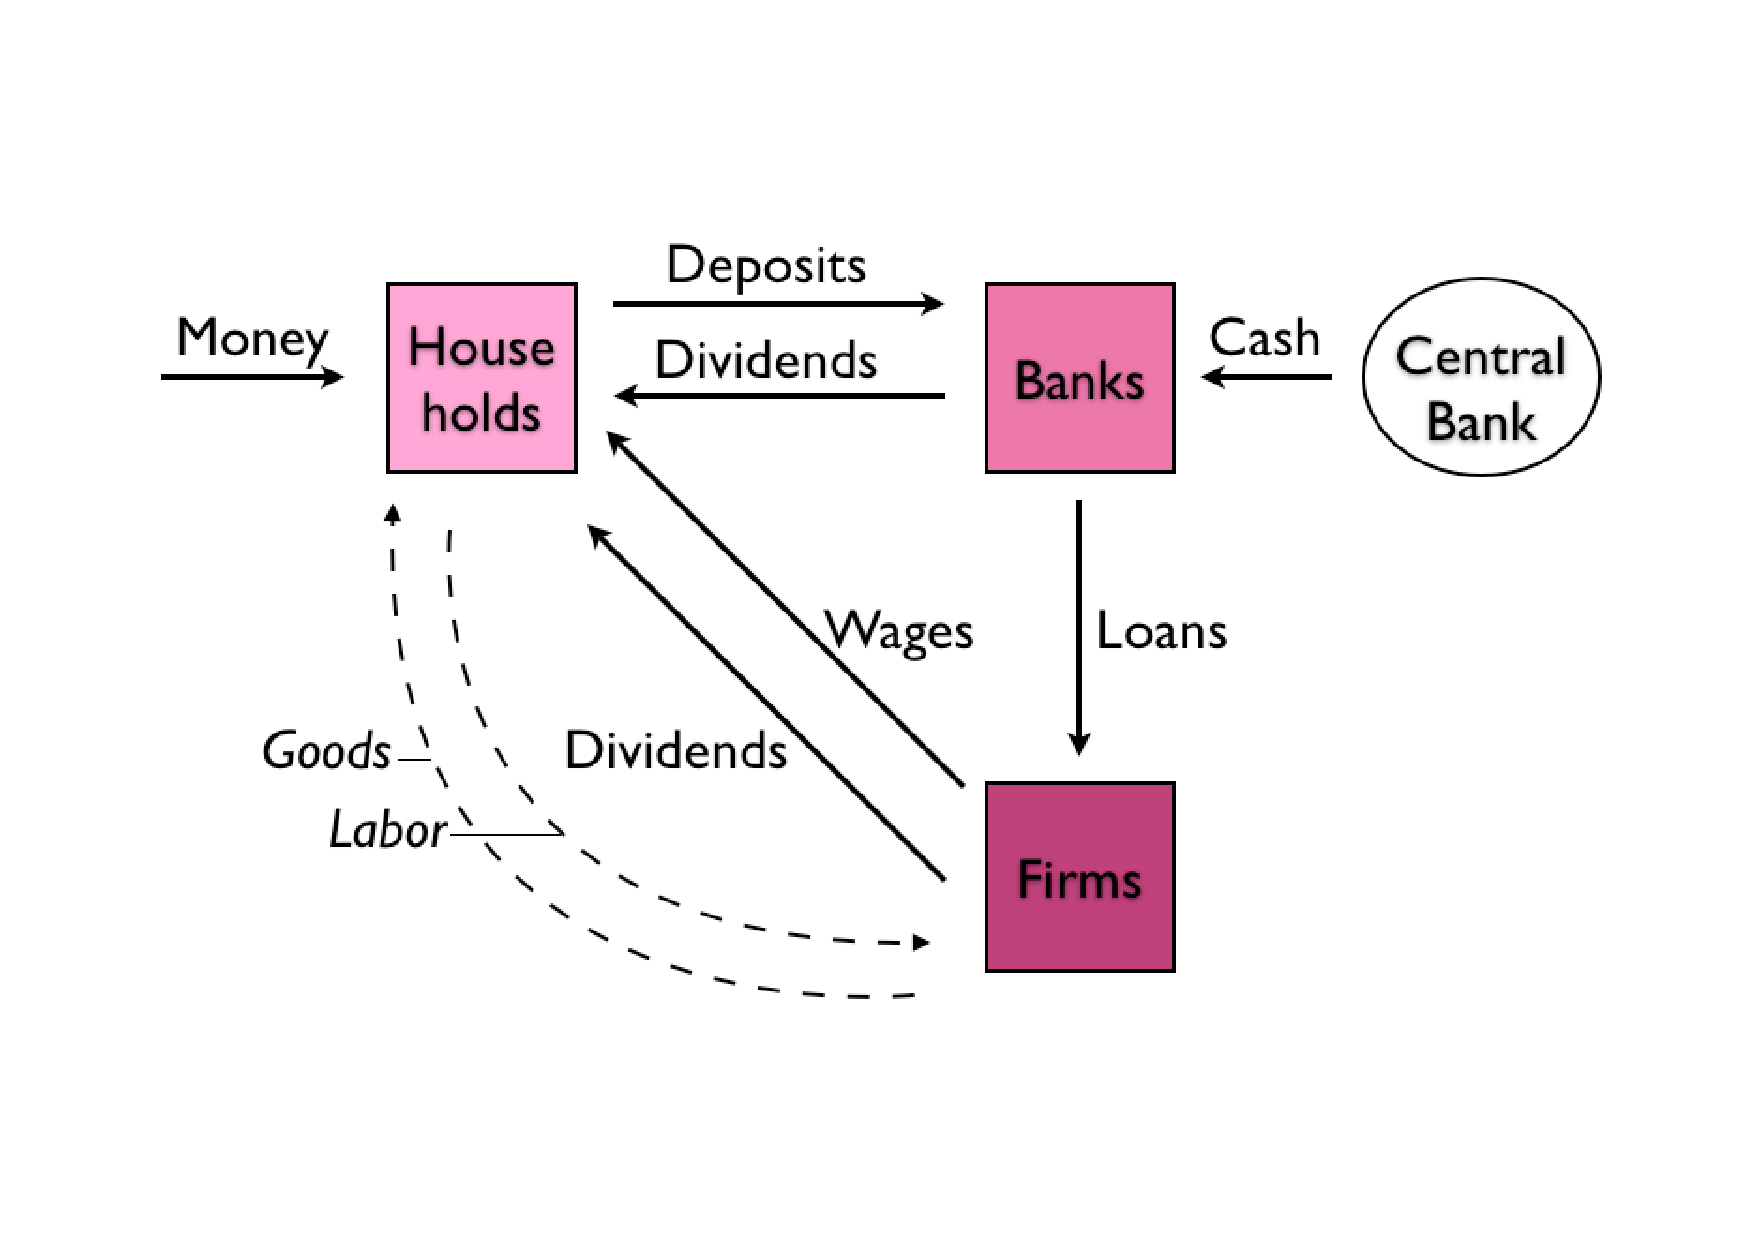
\includegraphics[width=1.0\textwidth]{P_SchorfMod} 
\end{center} 
\caption[CIA model illustration]{Continuous lines show the circulation of nominal funds, while dashed lines show the flow of real variables.} 
\end{figure}\\

The economy is made up of three central agents and one secondary agent: households, firms and banks (representing the financial sector), and a monetary authority which plays a minor role. Households maximize their utility function which depends on consumption, $C_t$, and hours worked, $H_t$, while deciding how much money to hold next period in cash, $M_{t+1}$ and how much to deposit at the bank, $D_t$, in order to earn $R_{H,t}-1$ interest. Households therefore solve the problem
\begin{eqnarray*}
\substack{\max \\ \{C_t,H_t,M_{t+1},D_t\}} & \mathbb{E}_0 \left[ \sum_{t=0}^\infty \beta^t \left[ (1-\phi) \ln C_t + \phi \ln (1-H_t) \right] \right] \\
\textrm{s.t.} & P_t C_t \leq M_t - D_t + W_t H_t \\
& 0 \leq D_t \\
& M_{t+1} = (M_t - D_t + W_tH_t - P_tC_t) + R_{H,t}D_t + F_t + B_t
\end{eqnarray*}
where the second equation spells out the cash in advance constraint including wage revenues, the third the inability to borrow from the bank and the fourth the intertemporal budget constraint emphasizing that households accumulate the money that remains after bank deposits and purchases on goods are deducted from total inflows made up of the money they receive from last period's cash balances, wages, interests, as well as dividends from firms, $F_t$, and from banks, $B_t$, which in both cases are made up of net cash inflows defined below. \\

Banks, on their end, receive cash deposits from households and a cash injection, $X_t$ from the central bank (which equals the net change in nominal money balances, $M_{t+1}-M_t$). It uses these funds to disburse loans to firms, $L_t$, on which they make a net return of $R_{F,t}-1$. Of course, banks are constrained in their loans by a credit market equilibrium condition $L_t \leq X_t + D_t$. Finally, bank dividends, $B_t$ are simply equal to $D_t + R_{F,t}L_t - R_{H,t}D_t - L_t + X_t$. \\

Finally, firms maximize the net present value of future dividends (discounted by the marginal utility of consumption, since they are owned by households) by choosing dividends, next period's capital stock, $K_{t+1}$, labor demand, $N_t$, and loans. Its problem is summarized by
\begin{eqnarray*}
\substack{\max \\ \{F_t,K_{t+1},N_{t},L_t\}} & \mathbb{E}_0 \left[ \sum_{t=0}^\infty \beta^{t+1} \frac{F_t}{C_{t+1}P_{t+1}} \right] \\
\textrm{s.t.} & F_t \leq L_t + P_t \left[ K_t^\alpha (A_t N_t)^{1-\alpha} - K_{t+1} + (1-\delta)K_t \right] - W_tN_t-L_tR_{F,t} \\
& W_tN_t \leq L_t\\
\end{eqnarray*}
where the second equation makes use of the production function \mbox{$Y_t = K_t^\alpha (A_t N_t)^{1-\alpha}$} and the real aggregate accounting constraint (goods market equilibrium) \mbox{$C_t + I_t = Y_t$}, where $I_t=K_{t+1} - (1-\delta)K_t$, and where $\delta$ is the rate of depreciation. Note that it is the firms that engage in investment in this model, by trading off investment for dividends to consumers. The third equation simply specifies that bank loans are used to pay for wage costs. \\

To close the model, we add the usual labor and money market equilibrium equations, $H_t= N_t$ and $P_tC_t=M_t + X_t$, as well as the condition that $R_{H,t}=R_{F,t}$ due to the equal risk profiles of the loans.\\

More importantly, we add a stochastic elements to the model. The model allows for two sources of perturbations, one real, affecting technology and one nominal, affecting the money stock. These important equations are
\[
\ln A_t = \gamma + \ln A_{t-1} + \epsilon_{A,t}, \qquad \epsilon_{A,t} \thicksim N(0,\sigma_A^2)
\]
and

\[
\ln m_t = (1-\rho)\ln m^* + \rho \ln m_{t-1} + \epsilon_{M,t}, \qquad \epsilon_{M,t} \thicksim N(0,\sigma_M^2)
\]
where $m_t \equiv M_{T+1}/M_t$ is the growth rate of the money stock. Note that theses expressions for trends are not written in the most straightforward manner nor very consistently. But we reproduced them never-the-less to make it easier to compare this example to the original paper. \\

The first equation is therefore a unit root with drift in the log of technology, and the second an autoregressive stationary process in the growth rate of money, but an AR(2) with a unit root in the log of the level of money. This can be seen from the definition of $m_t$ which can be rewritten as $\ln M_{t+1} = \ln M_t + \ln m_t$.\footnote{Alternatively, we could have written the AR(2) process in state space form and realized that the system has an eigenvalue of one. Otherwise said, one is a root of the second order autoregressive lag polynomial. As usual, if the logs of a variable are specified to follow a unit root process, the rate of growth of the series is a stationary stochastic process; see \citet{Hamilton1994}, chapter 15, for details.}\\

When the above functions are maximized, we obtain the following set of first order and equilibrium conditions. We will not dwell on the derivations here, to save space, but encourage you to browse \citet{CogleyNason1994} for additional details. We nonetheless give a brief intuitive explanation of each equation. The system comes down to
\begin{eqnarray*}
\mathbb{E}_{t}\bigg\{-\widehat{P}_{t}/\left[ \widehat{C}_{t+1}\widehat{P}_{t+1}m_{t}%
\right]\bigg\}&=&\beta e^{-\alpha (\gamma +\epsilon_{A,t+1})}P_{t+1}\Big[\alpha\widehat{K}_{t}^{\alpha -1}N_{t+1}^{1-\alpha }+
(1-\delta )\Big]\\
&&/\left[ 
\widehat{c}_{t+2}\widehat{P}_{t+2}m_{t+1}\right] \bigg\}\\
\widehat{W}_{t}&=&\widehat{L}_{t}/N_{t}\\
\frac{\phi }{1-\phi }\left[ \widehat{C}_{t}\widehat{P}_{t}/\left(
1-N_{t}\right) \right]&=&\widehat{L}_{t}/N_{t}\\
R_{t}&=&(1-\alpha )\widehat{P}_{t}e^{-\alpha (\gamma +\epsilon_{A,t+1})}\widehat{K}_{t-1}^{\alpha}N_{t}^{-\alpha }/\widehat{W}_{t}\\
\left[ \widehat{C}_{t}\widehat{P}_{t}\right] ^{-1}&=&\beta \left[ \left(
1-\alpha \right) \widehat{P}_{t}e^{-\alpha (\gamma +\epsilon_{A,t+1})}\widehat{K}_{t-1}^{\alpha}N_{t}^{1-\alpha }
\right]\\
&& \times  \mathbb{E}_{t}\left[\widehat{L}_{t}m_{t}\widehat{C}_{t+1}\widehat{P}_{t+1}\right] ^{-1}\\
\widehat{C}_t+\widehat{K}_t &=& e^{-\alpha(\gamma+\epsilon_{A,t})}\widehat{K}_{t-1}^\alpha N^{1-\alpha}+(1-\delta)e^{-(\gamma+\epsilon_{A,t})}\widehat{K}_{t-1}\\
\widehat{P}_t\widehat{C} &=& m_t\\
m_t-1+\widehat{D}_t &=& \widehat{L}_t\\
\widehat{Y}_t &=& \widehat{K}_{t-1}^\alpha N^{1-\alpha}e^{-\alpha (\gamma+\epsilon_{A,t})}\\
\ln(m_t) &=& (1-\rho)\ln(m^\star) + \rho\ln(m_{t-1})+\epsilon_{M,t}\\
\frac{A_t}{A_{t-1}}  \equiv  dA_t & = & \exp( \gamma + \epsilon_{A,t})\\
Y_t/Y_{t-1} &=& e^{\gamma+\epsilon_{A,t}}\widehat{Y}_t/\widehat{Y}_{t-1}\\
P_t/P_{t-1} &=& (\widehat{P}_t/\widehat{P}_{t-1})(m_{t-1}/e^{\gamma+\epsilon_{A,t}})
\end{eqnarray*}
where, importantly, hats over variables no longer mean deviations from steady state, but instead represent variables that have been made stationary. We come back to this important topic in details in section \ref{sec:nonstat} below. For now, we pause a moment to give some intuition for the above equations. In order, these equations correspond to:
\begin{enumerate}
\item The Euler equation in the goods market, representing the tradeoff to the economy of moving consumption goods across time.
\item The firms' borrowing constraint, also affecting labor demand, as firms use borrowed funds to pay for labor input.
\item The intertemporal labor market optimality condition, linking labor supply, labor demand, and the marginal rate of substitution between consumption and leisure. 
\item The equilibrium interest rate in which the marginal revenue product of labor equals the cost of borrowing to pay for that additional unit of labor.
\item The Euler equation in the credit market, which ensures that giving up one unit of consumption today for additional savings equals the net present value of future consumption.
\item The aggregate resource constraint.
\item The money market equilibrium condition equating nominal consumption demand to money demand to money supply to current nominal balances plus money injection. 
\item The credit market equilibrium condition.
\item The production function.
\item The stochastic process for money growth.
\item The stochastic process for technology.
\item The relationship between observable variables and stationary variables; more details on these last two equations appear in the following section. 
\end{enumerate}

\subsection{Declaring variables and parameters}
This block of the .mod file follows the usual conventions and would look like:\\
\\
\texttt{var m P c e W R k d n l Y\_obs P\_obs y dA; \\
varexo e\_a e\_m;\\
\\
parameters alp, bet, gam, mst, rho, psi, del;}\\
\\
where the choice of upper and lower case letters is not significant, the first set of endogenous variables, up to $l$, are as specified in the model setup above, and where the last five variables are defined and explained in more details in the section below on declaring the model in Dynare. The exogenous variables are as expected and concern the shocks to the evolution of technology and money balances. \\

\subsection{The origin of non-stationarity} \label{sec:nonstat}
The problem of non-stationarity comes from having stochastic trends in technology and money. The non-stationarity comes out clearly when attempting to solve the model for a steady state and realizing it does not have one. It can be shown that when shocks are null, real variables grow with $A_t$ (except for labor, $N_t$, which is stationary as there is no population growth), nominal variables grow with $M_t$ and prices with $M_t/A_t$. \textbf{Detrending} therefore involves the following operations (where hats over variables represent stationary variables): for real variables, $\hat q_t=q_t/A_t$, where $q_t = [y_t, c_t, i_t, k_{t+1} ]$. For nominal variables, $\hat{Q}_t = Q_t/M_t$, where $Q_t = [ d_t, l_t, W_t ]$. And for prices, $\hat P_t = P_t \cdot A_t / M_t$. \\

\subsection{Stationarizing variables}
Let's illustrate this transformation on output, and leave the transformations of the remaining equations as an exercise, if you wish (\citet{CogleyNason1994} includes more details on the transformations of each equation). We stationarize output by dividing its real variables (except for labor) by $A_t$. We define $\widehat{Y}_t$ to equal $Y_t / A_t$ and $\widehat{K}_t$ as $K_t / A_t$. \textsf{\textbf{NOTE!}} Recall from section \ref{sec:modspe} in chapter \ref{ch:solbase}), that in Dynare variables take the time subscript of the period in which they are decided (in the case of the capital stock, today's capital stock is a result of yesterday's decision). Thus, in the output equation, we should actually work with $\widehat{K}_{t-1}=K_{t-1} / A_{t-1}$. The resulting equation made up of stationary variables is
\begin{eqnarray*}
\frac{Y_t}{A_t} & = & \left( \frac{K_{t-1}}{A_{t-1}} \right)^\alpha A_t^{1-\alpha} N_t^{1-\alpha} A_t^{-1} A_{t-1}^\alpha \\
\widehat{Y}_t & = & \widehat{K}_{t-1}^\alpha N_t^{1-\alpha} \left( \frac{A_t}{A_{t-1}} \right)^{-\alpha} \\
& = & \widehat{K}_{t-1}^\alpha N_t^{1-\alpha} \exp(-\alpha (\gamma + \epsilon_{A,t}))
\end{eqnarray*}
where we go from the second to the third line by taking the exponential of both sides of the equation of motion of technology.\\

The above is the equation we retain for the .mod file of Dynare into which we enter:\\
\\
\texttt{y=k(-1)\textasciicircum alp*n\textasciicircum (1-alp)*exp(-alp*(gam+e\_a))}\\
\\

The other equations are entered into the .mod file after transforming them in exactly the same way as the one above. A final transformation to consider, that turns out to be useful since we often deal with the growth rate of technology, is to define \\
\\
\texttt{dA = exp(gam+e\_a)}\\
\\
by simply taking the exponential of both sides of the stochastic process of technology defined in the model setup above. \\

\subsection{Linking stationary variables to the data}
And finally, we must make a decision as to our \textbf{non-stationary observations}. We could simply stationarize them by \textbf{working with rates of growth} (which we know are constant). In the case of output, the observable variable would become $Y_t /Y_{t-1}$. We would then have to relate this observable, call it $gy\_{obs}$, to our (stationary) model's variables $\widehat Y_t$ by using the definition that $ \widehat{Y}_t \equiv Y_t/ A_t$. Thus, we add to the model block of the .mod file: \\
\\
\texttt{gy\_obs = dA*y/y(-1);}\\
\\
where, the $y$ of the .mod file are the stationary $\widehat Y_t$.\\

But, we could also \textbf{work with non-stationary data in levels}. This complicates things somewhat, but illustrates several features of Dynare worth highlighting; we therefore follow this path in the remainder of the example. The result is not very different, though, from what we just saw above. The goal is to add a line to the model block of our .mod file that relates the non stationary observables, call them $Y_{obs}$, to our stationary output, $\widehat Y_t$. We could simply write $Y_{obs} = \widehat Y_t A_t$. But since we don't have an $A_t$ variable, but just a $dA_t$, we we-write the above relationship in ratios. To the .mod file, we therefore add:\\
\\
\texttt{Y\_obs/Y\_obs(-1) = dA*y/y(-1);}\\
\\
We of course do the same for prices, our other observable variable, except that we use the relationship $P_{obs} = \widehat P_t M_t/A_t$ as noted earlier. The details of the correct transformations for prices are left as an exercise and can be checked against the results below.\\

\subsection{The resulting model block of the .mod file}

\texttt{model;\\
dA = exp(gam+e\_a);\\
log(m) = (1-rho)*log(mst) + rho*log(m(-1))+e\_m;\\
-P/(c(+1)*P(+1)*m)+bet*P(+1)*(alp*exp(-alp*(gam+log(e(+1))))*k\textasciicircum (alp-1)\\
*n(+1)\textasciicircum (1-alp)+(1-del)*exp(-(gam+log(e(+1)))))/(c(+2)*P(+2)*m(+1))=0;\\
W = l/n;\\
-(psi/(1-psi))*(c*P/(1-n))+l/n = 0;\\
R = P*(1-alp)*exp(-alp*(gam+e\_a))*k(-1)\textasciicircum alp*n\textasciicircum (-alp)/W;\\
1/(c*P)-bet*P*(1-alp)*exp(-alp*(gam+e\_a))*k(-1)\textasciicircum alp*n\textasciicircum (1-alp)/\\
(m*l*c(+1)*P(+1)) = 0;\\
c+k = exp(-alp*(gam+e\_a))*k(-1)\textasciicircum alp*n\textasciicircum (1-alp)+(1-del)\\
*exp(-(gam+e\_a))*k(-1);\\
P*c = m;\\
m-1+d = l;\\
e = exp(e\_a);\\
y = k(-1)\textasciicircum alp*n\textasciicircum (1-alp)*exp(-alp*(gam+e\_a));\\
Y\_obs/Y\_obs(-1) = dA*y/y(-1);\\
P\_obs/P\_obs(-1) = (p/p(-1))*m(-1)/dA;\\
end;}\\
\\
where, of course, the input conventions, such as ending lines with semicolons and indicating the timing of variables in parentheses, are the same as those listed in chapter \ref{ch:solbase}. \\

\textsf{\textbf{TIP!}} In the above model block, notice that what we have done is in fact relegated the non-stationarity of the model to just the last two equations, concerning the observables which are, after all, non-stationary. The problem that arises, though, is that we cannot linearize the above system in levels, as the last two equations don't have a steady state. If we first take logs, though, they become linear and it doesn't matter anymore where we calculate their derivative when taking a Taylor expansion of all the equations in the system. Thus, \textbf{when dealing with non-stationary observations, you must log-linearize your model} (and not just linearize it); this is a point to which we will return later. 

\subsection{Declaring observable variables}
We begin by declaring which of our model's variables are observables. In our .mod file we write\\
\\
\texttt{varobs P\_obs Y\_obs;}\\
\\
to specify that our observable variables are indeed $P\_obs$ and $Y\_obs$ as noted in the section above. \textsf{\textbf{NOTE!}} Recall from earlier that the number of observed variables must be smaller or equal to the number of shocks such that the model be estimated. If this is not the case, you should add measurement shocks to your model where you deem most appropriate. \\

\subsection{Declaring trends in observable variables}

Recall that we decided to work with the non-stationary observable variables in levels. Both output and prices exhibit stochastic trends. This can be seen explicitly by taking the difference of logs of output and prices to compute growth rates. In the case of output, we make use of the usual (by now!) relationship $Y_t=\widehat Y_t \cdot A_t$. Taking logs of both sides and subtracting the same equation scrolled back one period, we find:
\[
\Delta \ln Y_t = \Delta \ln \widehat Y_t + \gamma + \epsilon_{A,t}
\]
emphasizing clearly the drift term $\gamma$, whereas we know $\Delta \ln \widehat Y_t$ is stationary in steady state. \\

In the case of prices, we apply the same manipulations to show that:
\[
\Delta \ln P_t = \Delta \ln \widehat P_t + \ln m_{t-1} - \gamma - \epsilon_{A,t}
\]

Note from the original equation of motion of $\ln m_t$ that in steady state, $\ln m_t=\ln m^*$, so that the drift terms in the above equation are $\ln m^* - \gamma$.\footnote{This can also be see from substituting for $\ln m_{t-1}$ in the above equation with the equation of motion of $\ln m_t$ to yield: $\Delta \ln P_t = \Delta \ln \widehat P_t + \ln m^* + \rho(\ln m_{t-2}-\ln m^*) + \epsilon_{M,t} - \gamma - \epsilon_{A,t}$ where all terms on the right hand side are constant, except for $\ln m^*$ and $\gamma$.} \\

In Dynare, any trends, whether deterministic or stochastic (the drift term) must be declared up front. In the case of our example, we therefore write (in a somewhat cumbersome manner)\\
\\
\texttt{observation\_trends;\\
P\_obs (log(mst)-gam);\\
Y\_obs (gam);\\
end;}\\

In general, the command \texttt{observation\_trends} specifies linear trends as a function of model parameters for the observed variables in the model.\\

\subsection{Declaring unit roots in observable variables}

And finally, since P\_obs and Y\_obs inherit the unit root characteristics of their driving variables, technology and money, we must tell Dynare to use a diffuse prior (infinite variance) for their initialization in the Kalman filter. Note that for stationary variables, the unconditional covariance matrix of these variables is used for initialization. The algorithm to compute a true diffuse prior is taken from \citet{DurbinKoopman2001}. To give these instructions to Dynare, we write in the .mod\\
\\
\texttt{unit\_root\_vars P\_obs Y\_obs;}\\
\\
\textsf{\textbf{NOTE!}} You don't need to declare unit roots for any non-stationary model. Unit roots are only related to stochastic trends. You don't need to use a diffuse initial condition in the case of a deterministic trend, since the variance is finite.\\

\subsection{Specifying the steady state}
Declaring the steady state is just as explained in details and according to the same syntax explained in chapter \ref{ch:solbase}, covering the \texttt{initval}, \texttt{steady} and \texttt{check} commands. In chapter \ref{ch:estbase}, section \ref{sec:ssest}, we also discussed the usefulness of providing an external Matlab file to solve for the steady state. In this case, you can find the corresponding steady state file in the \textsl{models} folder under \textsl{UserGuide}. The file is called \textsl{fs2000ns\_steadystate.m}. There are some things to notice. First, the output of the function is the endogenous variables at steady state, the \texttt{ys} vector. The \texttt{check=0} limits steady state values to real numbers. Second, notice the declaration of parameters at the beginning; intuitive, but tedious... This functionality may be updated in later versions of Dynare. Third, note that the file is really only a sequential set of equalities, defining each variable in terms of parameters or variables solved in the lines above. So far, nothing has changed with respect to the equivalent file of chapter \ref{ch:estbase}. The only novelty is the declaration of the non-stationary variables, $P\_obs$ and $Y\_obs$ which take the value of 1. This is Dynare convention and must be the case for all your non-stationary variables. 

\subsection{Declaring priors}
We expand our .mod file with the following information: \\
\\
\texttt{estimated\_params;\\
alp, beta\_pdf, 0.356, 0.02; \\ 
bet, beta\_pdf, 0.993, 0.002; \\
gam, normal\_pdf, 0.0085, 0.003; \\
mst, normal\_pdf, 1.0002, 0.007; \\
rho, beta\_pdf, 0.129, 0.223;\\
psi, beta\_pdf, 0.65, 0.05;\\
del, beta\_pdf, 0.01, 0.005;\\
stderr e\_a, inv\_gamma\_pdf, 0.035449, inf;\\
stderr e\_m, inv\_gamma\_pdf, 0.008862, inf;\\
end;}\\
\\

\subsection{Launching the estimation}
We add the following commands to ask Dynare to run a basic estimation of our model:\\
\\
\texttt{estimation(datafile=fsdat,nobs=192,loglinear,mh\_replic=2000,\\
mode\_compute=4,mh\_nblocks=2,mh\_drop=0.45,mh\_jscale=0.65);}\\

\textsf{\textbf{NOTE!}} As mentioned earlier, we need to instruct Dynare to log-linearize our model, since it contains non-linear equations in non-stationary variables. A simple linearization would fail as these variables do not have a steady state. Fortunately, taking the log of the equations involving non-stationary variables does the job of linearizing them.\\

\subsection{The complete .mod file}
We have seen each part of the .mod separately; it's now time to get a picture of what the complete file looks like. For convenience, the file also appears in the \textsl{models} folder under \textsl{UserGuide} in your Dynare installation. The file is called \texttt{fs2000ns.mod}. \\
\\
\texttt{var m P c e W R k d n l Y\_obs P\_obs y dA; \\
varexo e\_a e\_m;\\
parameters alp, bet, gam, mst, rho, psi, del;\\
\\
model;\\
dA = exp(gam+e\_a);\\
log(m) = (1-rho)*log(mst) + rho*log(m(-1))+e\_m;\\
-P/(c(+1)*P(+1)*m)+bet*P(+1)*(alp*exp(-alp*(gam+log(e(+1))))\\
*k\textasciicircum (alp-1)*n(+1)\textasciicircum (1-alp)+(1-del)\\
*exp(-(gam+log(e(+1)))))/(c(+2)*P(+2)*m(+1))=0;\\
W = l/n;\\
-(psi/(1-psi))*(c*P/(1-n))+l/n = 0;\\
R = P*(1-alp)*exp(-alp*(gam+e\_a))*k(-1)\textasciicircum alp*n\textasciicircum (-alp)/W;\\
1/(c*P)-bet*P*(1-alp)*exp(-alp*(gam+e\_a))*k(-1)\textasciicircum alp*n\textasciicircum (1-alp)/\\(m*l*c(+1)*P(+1)) = 0;\\
c+k = exp(-alp*(gam+e\_a))*k(-1)\textasciicircum alp*n\textasciicircum (1-alp)+(1-del)\\*exp(-(gam+e\_a))*k(-1);\\
P*c = m;\\
m-1+d = l;\\
e = exp(e\_a);\\
y = k(-1)\textasciicircum alp*n\textasciicircum (1-alp)*exp(-alp*(gam+e\_a));\\
Y\_obs/Y\_obs(-1) = dA*y/y(-1);\\
P\_obs/P\_obs(-1) = (p/p(-1))*m(-1)/dA;\\
end;\\
\\
varobs P\_obs Y\_obs;\\
\\
observation\_trends;\\
P\_obs (log(mst)-gam);\\
Y\_obs (gam);\\
end;\\
\\
unit\_root\_vars P\_obs Y\_obs;\\
\\
initval;\\
k = 6;\\
m = mst;\\
P = 2.25;\\
c = 0.45;\\
e = 1;\\
W = 4;\\
R = 1.02;\\
d = 0.85;\\
n = 0.19;\\
l = 0.86;\\
y = 0.6;\\
dA = exp(gam);\\
end;\\
\\
// the above is really only useful if you want to do a stoch\_simul\\
// of your model, since the estimation will use the Matlab\\
// steady state file also provided and discussed above.\\
\\
steady;\\
\\
estimated\_params;\\
alp, beta\_pdf, 0.356, 0.02; \\ 
bet, beta\_pdf, 0.993, 0.002; \\
gam, normal\_pdf, 0.0085, 0.003; \\
mst, normal\_pdf, 1.0002, 0.007; \\
rho, beta\_pdf, 0.129, 0.223;\\
psi, beta\_pdf, 0.65, 0.05;\\
del, beta\_pdf, 0.01, 0.005;\\
stderr e\_a, inv\_gamma\_pdf, 0.035449, inf;\\
stderr e\_m, inv\_gamma\_pdf, 0.008862, inf;\\
end;\\
\\
estimation(datafile=fsdat,nobs=192,loglinear,mh\_replic=2000,\\
mode\_compute=4,mh\_nblocks=2,mh\_drop=0.45,mh\_jscale=0.65);}\\
\\

\subsection{Summing it up}
The explanations given above of each step necessary to translate the \citet{Schorfheide2000} example into language that Dynare can understand and process was quite lengthy and involved a slew of new commands and information. It may therefore be useful, to gain a ``bird's eyeview'' on what we have just accomplished, and summarize the most important steps at a high level. This is done in figure \ref{fig:estsumm}.\\
\begin{figure} \label{fig:estsumm}
\begin{center} 
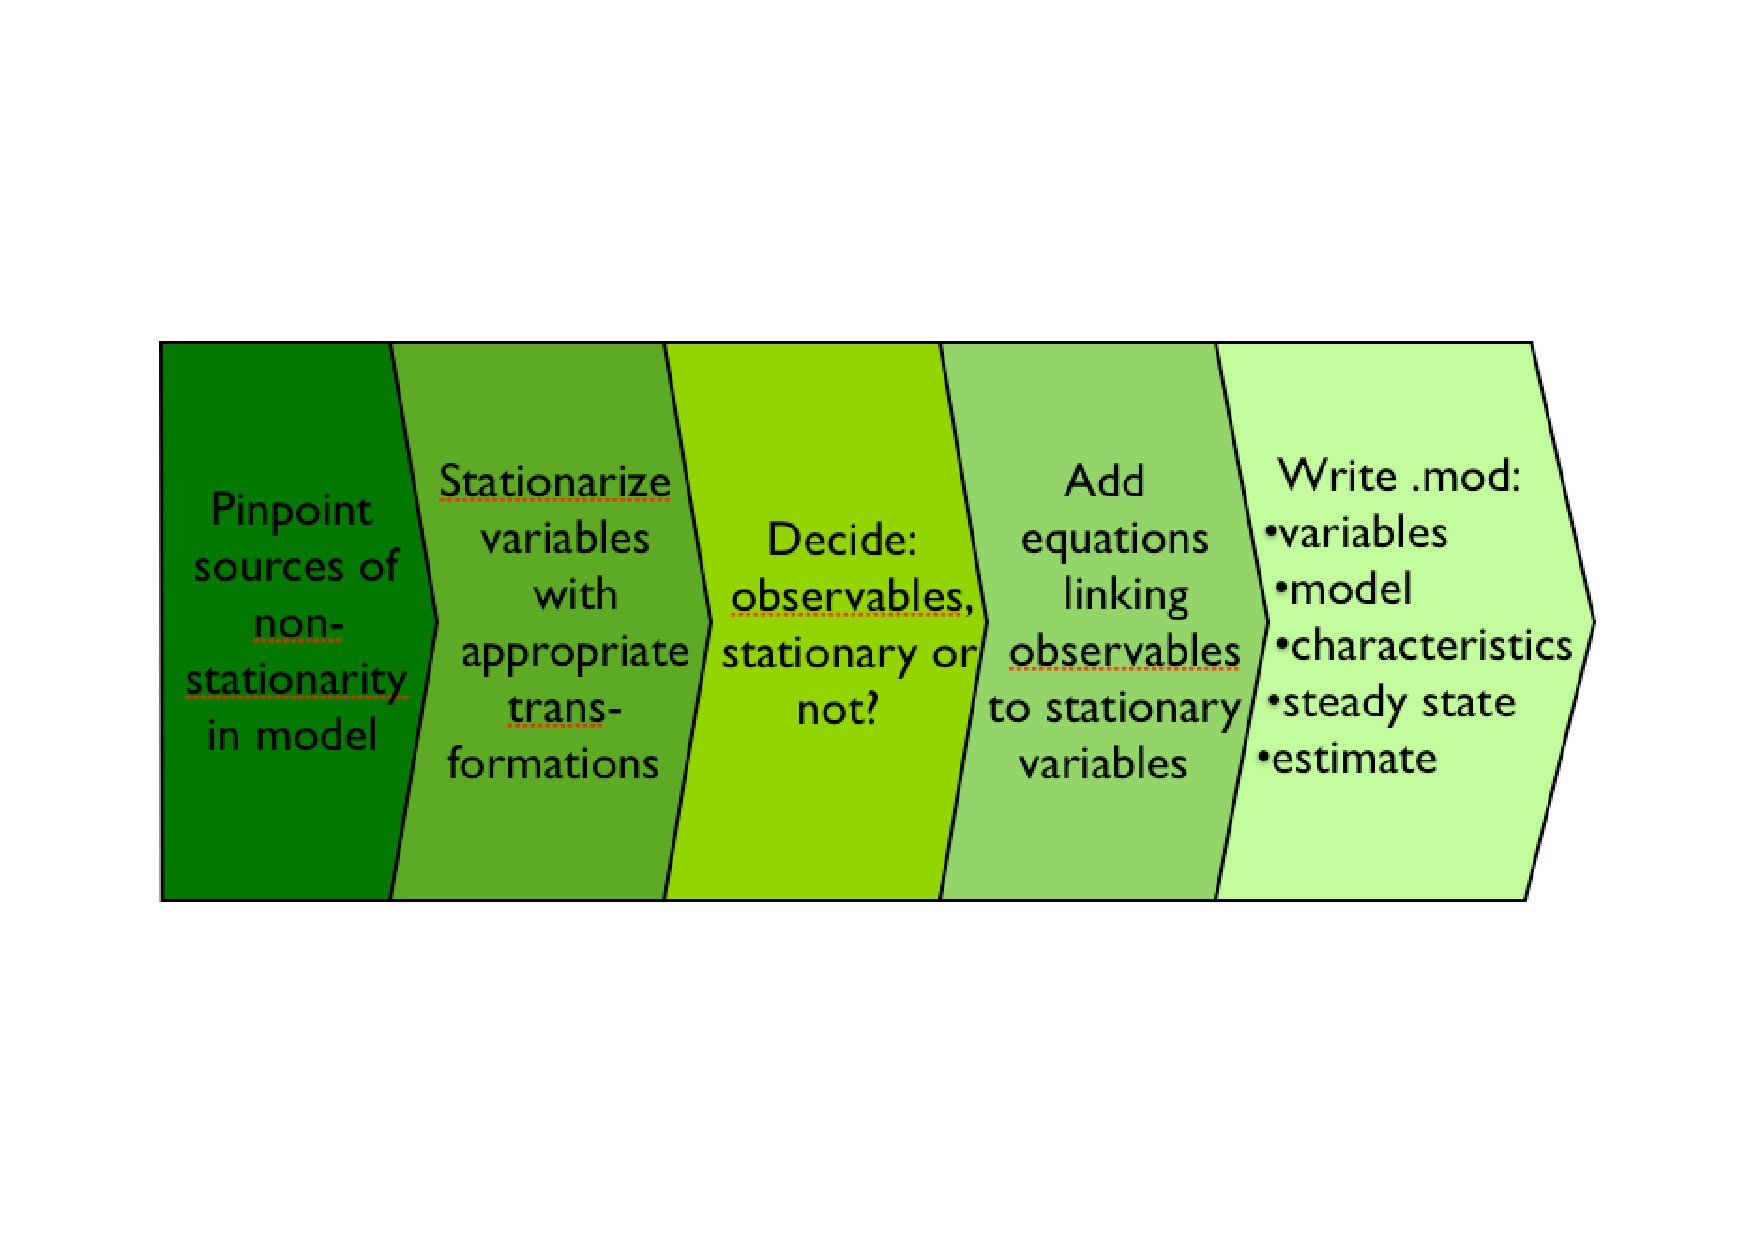
\includegraphics[width=1.0\textwidth]{P_flowest} 
\end{center} 
\caption[Steps of model estimation]{At a high level, there are five basic steps to translate a model into Dynare for successful estimation.} 
\end{figure}\\


\section{Comparing models based on their posterior distributions}
** TBD

\section{Where is your output stored?}
The output from estimation can be extremely varied, depending on the instructions you give Dynare. The \href{http://www.dynare.org/documentation-and-support/manual}{Reference Manual} overviews the complete set of potential output files and describes where you can find each one. 